% !TeX TS-program = xelatex
\documentclass[aspectratio=169, 12pt, xcolor=table]{beamer}
\usefonttheme{professionalfonts}
\usefonttheme{serif}
\usepackage[T1]{fontenc}
\usepackage{fontspec-xetex}

\usepackage{booktabs}
\usepackage{listings}
\usepackage{subcaption}

\setmainfont{Lato}

%\PassOptionsToPackage[more=table]{xcolor}

% Local configuration
\renewcommand{\figurename}{}
\DeclareCaptionFormat{custom}
{%
	\tiny #3
}
\captionsetup{format=custom}

% Title stuff
\title{Statistical Techniques}
\subtitle{Linear Regression}
\date{Week 05}
\author{Vassilis Markos, Mediterranean College}

\usetheme{streamline}
%\usepackage{/theme/beamerthemestreamline}

% Local Commands
\newcommand{\ohref}[1]{\href{#1}{\texttt{#1}}}
\def\sms#1{\smsgo#1\relax}
\def\smsgo#1.#2\relax{#1.{\scriptsize #2}}

% Code listings

\definecolor{codegreen}{rgb}{0,0.6,0}
\definecolor{codegray}{rgb}{0.5,0.5,0.5}
\definecolor{codepurple}{rgb}{0.58,0,0.82}
\definecolor{backcolour}{rgb}{0.95,0.95,0.92}

\lstdefinestyle{mystyle}{
	backgroundcolor=\color{backcolour},   
	commentstyle=\color{codegreen},
	keywordstyle=\color{magenta},
	numberstyle=\tiny\color{codegray},
	stringstyle=\color{codepurple},
	basicstyle=\ttfamily\footnotesize,
	breakatwhitespace=false,         
	breaklines=true,                 
	captionpos=b,                    
	keepspaces=true,                 
	numbers=left,                    
	numbersep=5pt,                  
	showspaces=false,                
	showstringspaces=false,
	showtabs=false,                  
	tabsize=2
}

\lstset{style=mystyle}

\begin{document}

	\begin{frame}
		\titlepage
	\end{frame}

	\begin{frame}{Contents}
		\tableofcontents
	\end{frame}

	\section{A Simple Example}\label{sec:descriptive-statistics}
	
	\sectionframe
	
	\begin{frame}[fragile]{Good (?) Ol' Cars\ldots}
		Consider the following simple car dataset about some 1973-74 models:
		
		\lstinputlisting[language=R, linerange={9-9}]{src/lg.Rmd}
		
		\begin{small}
		\begin{verbatim}
                  mpg  cyl disp  hp drat    wt  qsec vs am gear carb
Mazda RX4         21.0   6  160 110 3.90 2.620 16.46  0  1    4    4
Mazda RX4 Wag     21.0   6  160 110 3.90 2.875 17.02  0  1    4    4
Datsun 710        22.8   4  108  93 3.85 2.320 18.61  1  1    4    1
Hornet 4 Drive    21.4   6  258 110 3.08 3.215 19.44  1  0    3    1
Hornet Sportabout 18.7   8  360 175 3.15 3.440 17.02  0  0    3    2
Valiant           18.1   6  225 105 2.76 3.460 20.22  1  0    3    1
\end{verbatim}
		\end{small}
	\end{frame}

	\begin{frame}{What Affects \texttt{mpg}?}
		\begin{itemize}
			\item One valuable question might be which variables are correlated with which others and, more valuably, which ones predict others.
			\item One easy way to quick-check what goes on is to plot scatter plots of all data pairwise.
			\item The following command plots all such scatter plots twice (for $X,Y$ interchangeably) for \texttt{mpg} against all other dataset variables.
		\end{itemize}
	
		\lstinputlisting[language=R, linerange={12-12}]{src/lg.Rmd}
		
	\end{frame}


	\begin{frame}{What Affects \texttt{mpg}?}
		
		\begin{center}
			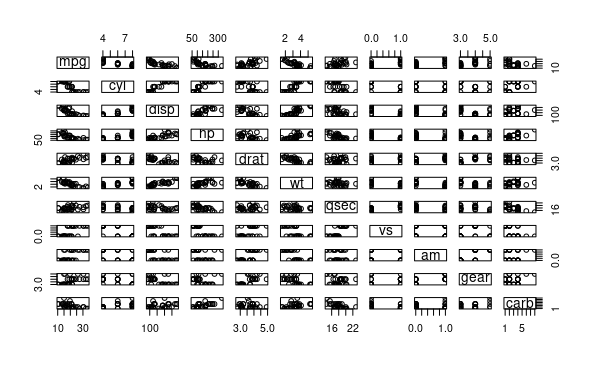
\includegraphics[width=0.75\textwidth]{img/pairs.png}
		\end{center}
		
	\end{frame}

	\begin{frame}{Okay, So\ldots What?}
		\begin{itemize}
			\item Take some time to meditate on the previous image\ldots
			\item Since the plot matrix is symmetric, focus either on the lower or the upper triangular part.
			\item One correlation that we might consider exploring further should be between \texttt{mpg} and \texttt{wt} (i.e., miles per gallon and weight in lbs).
			\item So, we can plot this one scatter plot separately:
		\end{itemize}
		
		\lstinputlisting[language=R, linerange={16-16}]{src/lg.Rmd}
		
	\end{frame}
	
	
	\begin{frame}{Okay, So\ldots What?}
		\begin{center}
			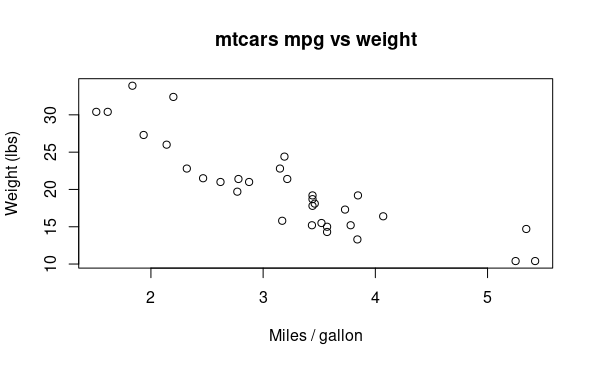
\includegraphics[width=0.75\textwidth]{img/mpgwt.png}
		\end{center}
	\end{frame}

	\begin{frame}{Among the Fogs of \texttt{mtcars}\ldots}
		\begin{itemize}
			\item \ldots a linear relationship between mpg and wt appears.
			\item So, how can we make sure that there actually is one?
			\item Here comes linear regression! A straight line has the shape of:
			\[y=\beta_0+\beta_1x.\]
			\item The thing in our case is that, evidently, the points in the previous plot do not form a straight line. We can capture this deviation from a purely straight line by introducing an error term:
			\[y=\beta_0+\beta_1x+\varepsilon.\]
		\end{itemize}
	\end{frame}

	\begin{frame}{Survival of the Fittest}
		\begin{itemize}
			\item Okay, but, this uncertainty introduces an infinity of different choices for $\beta_0,\beta_1$, i.e., an infinity of candidate straight lines.
			\item Which one to choose? (Any ideas?)\pause
			\item One criterion would be to minimise total error on each sample observation, i.e., for each estimated value of our model:
			\[\hat{y}_i=\beta_0+\beta_1x_i,\quad i=1,\ldots,n,\]
			we should compute and minimise the corresponding errors:
			\[\varepsilon_i=\hat{y}_i-y_i,\quad i=1,\ldots,n.\]
		\end{itemize}
	\end{frame}

	\begin{frame}{But, What to Minimise?}
		\begin{itemize}
			\item So, one approach here would be to minimise the total error:
			\[SE=\sum_{i=1}^n\varepsilon_i.\]
			\item Can you see the pitfall here?\pause
			\item While summing all errors, positive and negative values might cancel out, resulting to misleading results.
		\end{itemize}
	\end{frame}

	\begin{frame}{But, What to Minimise?}
		\begin{itemize}
			\item Another alternative would be to drop sign, i.e., compute and minimise:
			\[SAE=\sum_{i=1}^n\left|\varepsilon_i\right|.\]
			\item This resolves the previous issue of errors cancelling, but, mathematically, the absolute value function is inconvenient to work with (i.e., non-differentiable).
			\item So, we end up with:
			\[\boxed{SSE=\sum_{i=1}^n\varepsilon_i^2.}\]
		\end{itemize}
	\end{frame}


	\begin{frame}{The Linear Regression Model}
		\begin{itemize}
			\item Trying to minimise $SSE$ by common multivariate calculus techniques, we find that the optimal values for $\beta_0,\beta_1$ should be:
			\begin{align*}
				\hat{\beta}_0&=\overline{y}-\hat{\beta}\overline{x}\\
				\hat{\beta}_1&=\frac{\sum_{i=1}^n(x_i-\overline{x})(y_i-\overline{y})}{\sum_{i=1}^n(x_i-\overline{x})^2}
			\end{align*}
			\item The standard error of the above model is defined as the square root of $s^2$, where:
			\[s^2=\frac{SSE}{n-1}.\]
		\end{itemize}
	\end{frame}

	\begin{frame}[fragile]{Application on \texttt{mtcars}}
		
		\lstinputlisting[language=R, linerange={20-21}]{src/lg.Rmd}
		
		\begin{tiny}
\begin{verbatim}
Call:
lm(formula = mpg ~ wt, data = mtcars)

Residuals:
Min      1Q  Median      3Q     Max 
-4.5432 -2.3647 -0.1252  1.4096  6.8727 

Coefficients:
Estimate Std. Error t value Pr(>|t|)    
(Intercept)  37.2851     1.8776  19.858  < 2e-16 ***
wt           -5.3445     0.5591  -9.559 1.29e-10 ***
---
Signif. codes:  0 ‘***’ 0.001 ‘**’ 0.01 ‘*’ 0.05 ‘.’ 0.1 ‘ ’ 1

Residual standard error: 3.046 on 30 degrees of freedom
Multiple R-squared:  0.7528,    Adjusted R-squared:  0.7446 
F-statistic: 91.38 on 1 and 30 DF,  p-value: 1.294e-10
\end{verbatim}
		\end{tiny}
		
	\end{frame}


	\begin{frame}{Why $R^2$ and $p$-values?}
		\begin{itemize}
			\item As you might observe, the previous slide contains some statistical terms that ring a bell\ldots Can you suspect why?\pause
			\item In order to test the model's fitness, we perform a hypothesis testing, where we assume that the errors are normally distributed, with a mean value of zero, and use as a null hypothesis:
			\[H_0=\beta_1=0.\]
			\item That is, under the assumption that errors are normally distributed around zero, we assume that there is no linear relationship between our two variables.
		\end{itemize}
	\end{frame}

	
	\begin{frame}{Why $R^2$ and $p$-values?}
		\begin{itemize}
			\item Thus, we can use all our known hypothesis testing machinery to test whether or not a linear model is properly explaining the data we have at hand.
			\item For example, as with ANOVA, we have $R^2$ explain the percentage of variance in data captured by our model, since:
			\[R^2=\frac{SSR}{SST}=1-\frac{SSE}{SST}.\]
			\item Recall: $SSE$ is the errors sum of squares, $SSR$ is the regression sum of squares and $SST$ is the total sum of squares.
		\end{itemize}
	\end{frame}


	\begin{frame}{(Reminder) Errors}
		As a brief reminder, with our notation so far:
		\begin{align*}
			SST&=SSR+SSE\\
			SST&=\sum_{i=1}^n(\hat{y}_i-y_i)^2\\
			SSR&=\sum_{i=1}^n(\hat{y}_i-\overline{y})^2\\
			SSE&=\sum_{i=1}^n(y_i-\overline{y})^2\\
		\end{align*}
	\end{frame}


	\begin{frame}{So, How Does Our Model Look Like?}
		\begin{itemize}
			\item To plot our model over the scattered data points, we have to plot both one on top of the other.
			\item Remember to plot your variables the same way they appear in your model, i.e., $y$ against $x$, otherwise, you might get a non-sensical plot!
		\end{itemize}
		
		\lstinputlisting[language=R, linerange={25-26}]{src/lg.Rmd}
	\end{frame}


	\begin{frame}{Our Model!}
		\begin{center}
			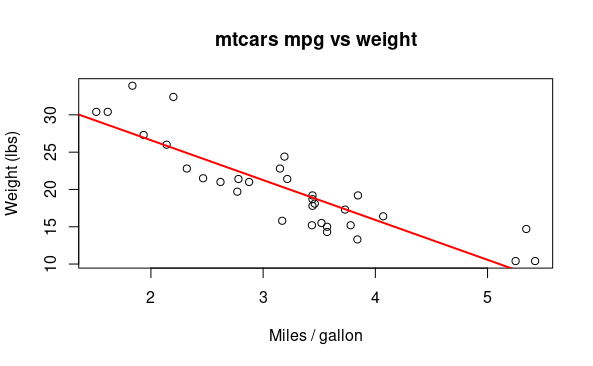
\includegraphics[width=0.75\textwidth]{img/model.png}
		\end{center}
	\end{frame}


	\begin{frame}{Further Model Evaluation}
		\begin{itemize}
			\item \textbf{Residuals vs Fitted} plots, which plot the predicted values versus the corresponding errors. Ideally, it should look like randomly arranged points with no significant patterns.
			\item \textbf{Normal Q-Q} plots, which show standardised residuals vs their theoretical values. Ideally, all points should like on the diagonal.
			\item \textbf{Scale-location} plots, which plots predicted against square root standardised errors.
			\item \textbf{Residuals-Leverage} plots, which identify points that might affect the regression line a lot.
		\end{itemize}
	\end{frame}

	\begin{frame}{Residuals vs Fitted}
		\begin{center}
			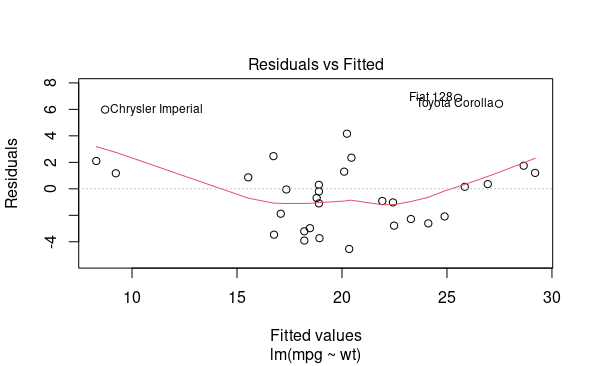
\includegraphics[width=0.75\textwidth]{img/rsdfit.png}
		\end{center}
	\end{frame}


	\begin{frame}{Normal Q-Q}
		\begin{center}
			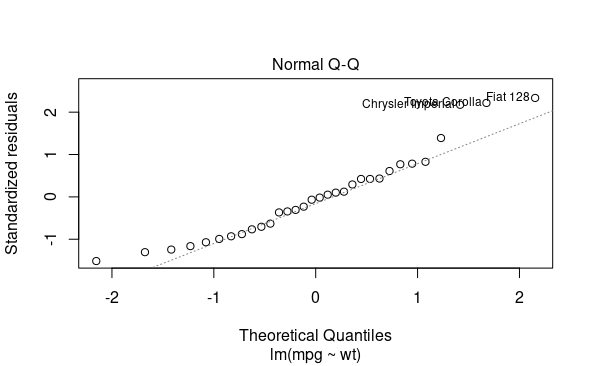
\includegraphics[width=0.75\textwidth]{img/qq.png}
		\end{center}
	\end{frame}


	\begin{frame}{Scale-Location}
		\begin{center}
			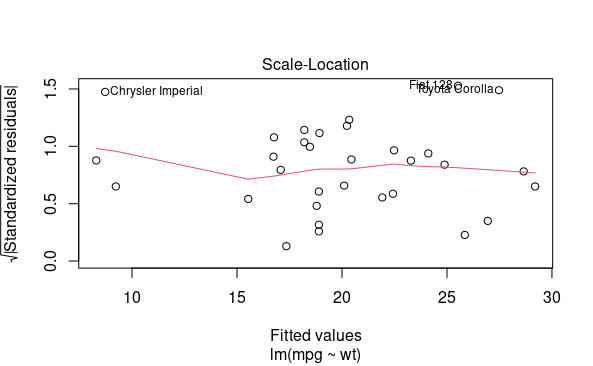
\includegraphics[width=0.75\textwidth]{img/sl.png}
		\end{center}
	\end{frame}


	\begin{frame}{Residuals vs Leverage}
		\begin{center}
			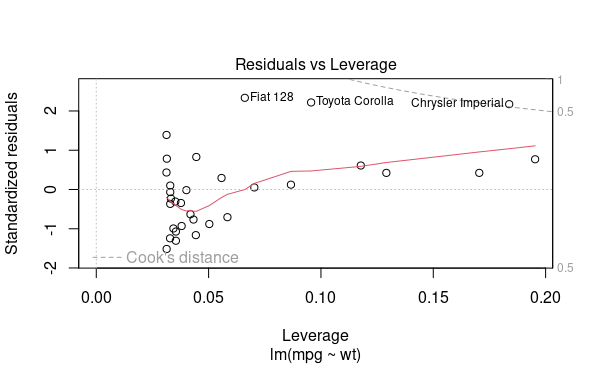
\includegraphics[width=0.75\textwidth]{img/rl.png}
		\end{center}
	\end{frame}

	\begin{frame}{Don't Rely Just on Regression!}
		\begin{center}
			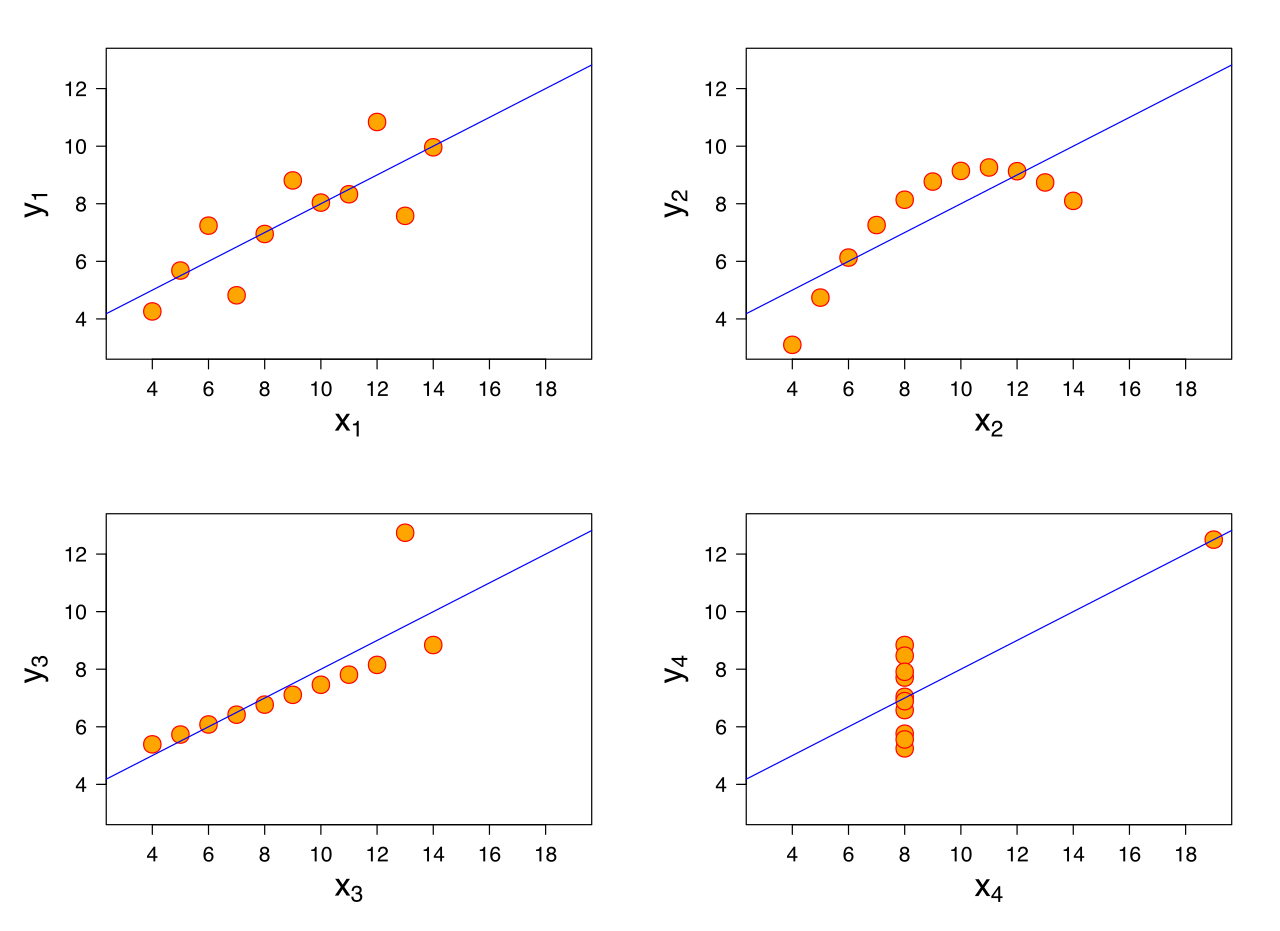
\includegraphics[width=0.5\textwidth]{img/anscombe.png}
		\end{center}
		{\tiny Source: \url{https://en.wikipedia.org/wiki/Linear_regression\#Least-squares_estimation_and_related_techniques}}
	\end{frame}
	
	
\end{document}